% Final presentation, team 8, Thursday 3 Dec 2026. 10 minutes in all: about 5 of slides, 5 of live demo.
% Same look as the NN-project deck: many short slides, little text, the speaker carries the talk.
% Style rules: one text size and one text colour everywhere; a title plus one to three short full
% sentences per slide; capital letter and full stop on every sentence; plain words; no numbers.
% Text is left-aligned and starts at the same height on every slide; only pictures are centred.
% Parts: vision.tex (Leonardo), app.tex (Ali). Who presents the opening and closing slides: to decide.
% Pictures: python slides/make_figures.py (needs the local paper/photos folder).
% Build: latexmk -pdf slides.tex
\documentclass[aspectratio=169,12pt]{beamer}

\usepackage[T1]{fontenc}
\usepackage{lmodern}
\usepackage{tikz}
\usetikzlibrary{arrows.meta,positioning}
\usepackage{qrcode}

% Look
\definecolor{ink}{HTML}{1F2328}
\definecolor{muted}{HTML}{6E7781}
\definecolor{faint}{HTML}{D0D7DE}
\definecolor{accent}{HTML}{0B5CAD}
\setbeamercolor{normal text}{fg=ink,bg=white}
\setbeamercolor{frametitle}{fg=ink}
\setbeamercolor{structure}{fg=accent}
\setbeamerfont{frametitle}{size=\Large,series=\bfseries}
\setbeamertemplate{navigation symbols}{}
\setbeamertemplate{itemize items}{\textcolor{muted}{--}}
\setbeamertemplate{frametitle}{\vspace{0.6em}\insertframetitle}
\setbeamertemplate{footline}{\hfill\textcolor{muted}{\scriptsize\insertframenumber}\hspace{1.2em}\vspace{0.8em}}
\setlength{\parskip}{0.5em}

% Every slide body: same size, same colour, same starting height.
\newcommand{\body}[1]{\vspace*{1.2em}{\large #1\par}\vfill}
% A centred picture, then the body text under it.
\newcommand{\withpic}[2]{\vspace*{1.2em}\begin{center}#1\end{center}\vspace{0.8em}{\large #2\par}\vfill}
% Pictures side by side, all with the same height.
\newcommand{\pic}[2][0.46\textheight]{\includegraphics[height=#1]{figures/#2}}
% Four pictures in a row.
\newcommand{\fit}[1]{\includegraphics[width=0.22\textwidth,height=0.42\textheight,keepaspectratio]{figures/#1}}

\tikzset{
  flow/.style={node distance=6mm, every node/.style={font=\large, align=center},
    >={Stealth[length=2.5mm]}},
  box/.style={draw=ink, rounded corners=2pt, minimum width=24mm, minimum height=14mm},
}

\begin{document}

% 1
\begin{frame}[plain]
  \vfill
  {\LARGE\bfseries AR Sudoku Solver\par}
  \vspace{1.5em}
  {\large Leonardo Tisato and Muhammad Ali Hassan.\par
  UIC, CS 415, 3 December 2026.\par}
  \vfill
\end{frame}

% 2
\begin{frame}{Goal}
  \withpic{\pic{goal.jpg}}{Point a phone at a Sudoku on paper, and the missing digits appear on the
  paper, all in the browser.}
\end{frame}

% 3
\begin{frame}{Pipeline}
  \withpic{%
  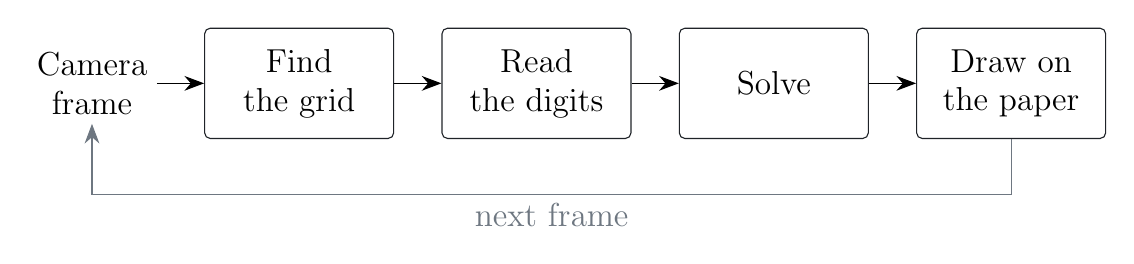
\begin{tikzpicture}[flow]
    \node (f) {Camera\\frame};
    \node[box, right=of f] (g) {Find\\the grid};
    \node[box, right=of g] (d) {Read\\the digits};
    \node[box, right=of d] (s) {Solve};
    \node[box, right=of s] (p) {Draw on\\the paper};
    \draw[->] (f) -- (g); \draw[->] (g) -- (d); \draw[->] (d) -- (s); \draw[->] (s) -- (p);
    \draw[->, muted] (p.south) -- ++(0,-7mm) -| node[pos=0.25, below] {next frame} (f.south);
  \end{tikzpicture}}{Every camera frame goes through four steps.}
\end{frame}

% Finding the grid, reading the digits, solving (slides 4-10). Presented by Leonardo.

% 4
\begin{frame}{Finding the grid}
  \withpic{\pic{grid_threshold.jpg}\hspace{1em}\pic{grid_contour.jpg}}{An adaptive threshold turns
  the ink white and the paper black. The grid is the largest contour with four corners.}
\end{frame}

% 5
\begin{frame}{Flattening the grid}
  \withpic{\pic{grid_contour.jpg}\hspace{1em}\pic{grid_lines.jpg}}{The four corners give a
  homography, which flattens the grid into a square. It is a Sudoku only if there is a line at every
  cell border.}
\end{frame}

% 6
\begin{frame}{Objects touching the grid}
  \withpic{\pic{merged_contour.jpg}\hspace{1em}\pic{merged_refined.jpg}}{When an object touches the
  grid, the contour goes around both. We start from the four corners of its convex hull, and move each
  corner a little at a time while the cell borders line up better.}
\end{frame}

% 7
\begin{frame}{Printed digits}
  \withpic{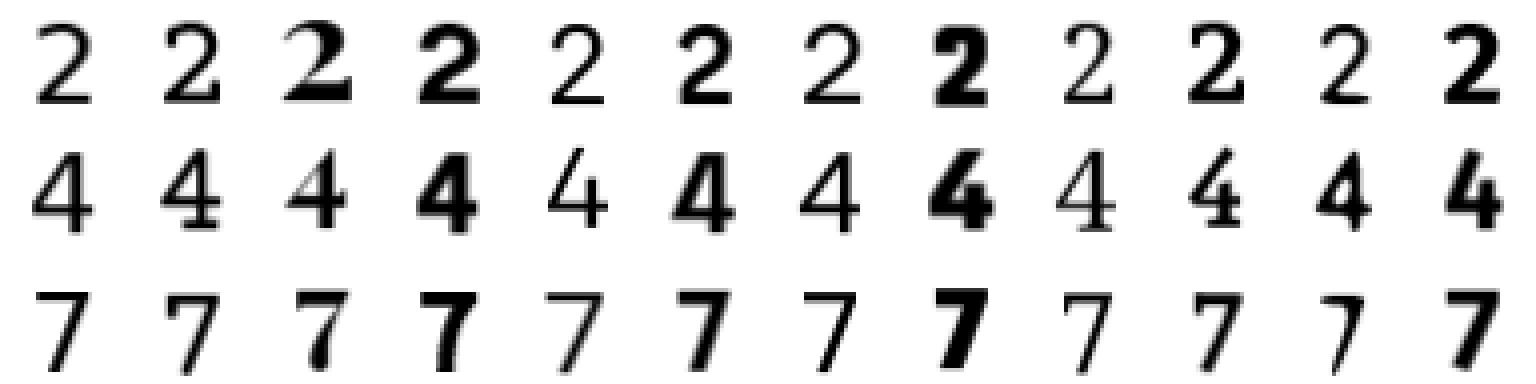
\includegraphics[width=0.6\textwidth]{figures/templates.png}}{Each digit is compared
  with the digits 1 to 9 in many fonts, and the best match gives the digit. We try the grid in four
  rotations: the one that matches best is the right way up.}
\end{frame}

% 8
\begin{frame}{Printed or handwritten}
  \withpic{\pic[0.4\textheight]{digits_flat.jpg}\hspace{1em}\pic[0.4\textheight]{digits_read.jpg}}%
  {A digit is printed if it matches a font well and is as dark and as tall as the other printed
  ones. Handwritten digits are described with HOG, a histogram of edge directions, and get the label
  of the closest MNIST digits.}
\end{frame}

% 9
\begin{frame}{Solving}
  \withpic{\pic{mistakes.jpg}}{Backtracking solves the puzzle from the printed digits. A
  proper Sudoku has only one solution, so a handwritten digit that differs from it is a mistake.}
\end{frame}

% 10
\begin{frame}{The order of the digits}
  \withpic{\pic{order.jpg}}{We show the digits in the order a person would find them, starting from
  the cells where only one digit fits.}
\end{frame}

% The app (slides 11-12). Presented by Ali. Draft by Leonardo: Ali, change anything.

% 11
\begin{frame}{Tracking}
  \body{Reading the digits is slow, so we read them only now and then. In the other frames we only
  follow the four corners, and smooth them so the digits do not shake.}
\end{frame}

% 12 (a phone screenshot would fit here)
\begin{frame}{The app}
  \body{%
  \begin{itemize}
    \item The app is a static web page, and our Python code runs inside it with Pyodide.
    \item The digits are drawn on a flat square, and the homography bends it onto the paper.
    \item Live shows the whole solution, Step one digit at a time.
    \item Without paper, a virtual board can be placed on a table or a wall.
  \end{itemize}}
\end{frame}


% 13
\begin{frame}{What works}
  \withpic{\fit{example_0383.jpg}\hspace{0.5em}\fit{example_0388.jpg}\hspace{0.5em}%
  \fit{example_0392.jpg}\hspace{0.5em}\fit{example_0416.jpg}}%
  {It works on rotated and tilted paper, in shadows and on different backgrounds. Pencil and pen
  digits are read too.}
\end{frame}

% 14
\begin{frame}{What does not work}
  \withpic{\pic{example_0402.jpg}\hspace{1em}\pic{example_0397.jpg}}{A bent sheet fails: one
  homography can only flatten a flat sheet. It also fails when the border is covered, and it
  sometimes misreads a handwritten digit.}
\end{frame}

% 15 (the backup video goes here as a link, in case the live demo breaks)
\begin{frame}{Demo}
  \body{Live demo.}
\end{frame}

% 16
\begin{frame}{Try it}
  \withpic{\qrcode[height=0.4\textheight]{https://alihassanmirza1.github.io/AR-Sudoku-Solver-with-Computer-Vision/}}%
  {Open the app on your phone: alihassanmirza1.github.io/AR-Sudoku-Solver-with-Computer-Vision.}
\end{frame}

\end{document}
